% !TeX spellcheck = en_US
% !TeX encoding = UTF-8

% COMPILE WITH:
% `latexmk`
% You need lualatex and biber (in all TeXLive distributions)

\documentclass[
    numbers=noenddot,
    %listof=totoc,
    parskip=half-,
    fontsize=12pt,
    paper=a4,
    oneside,
    titlepage,
    bibliography=totoc,
    chapterprefix=false,
%    draft
]{scrbook}

% use lualatex or xelatex
\usepackage{fontspec}
\usepackage{graphicx}
\usepackage[doublespacing]{setspace}

\usepackage{float} % Add this line in the preamble

% better language support
\usepackage{polyglossia}
\setdefaultlanguage{english}
\setotherlanguage{german}

\usepackage{tocbasic}
\usepackage{booktabs}
\usepackage{multicol}
\usepackage{multirow}

\usepackage[]{scrlayer-scrpage}

% better bibliography (biblatex style)
% use biber to compile
\usepackage[citestyle=alphabetic, bibstyle=alphabetic, sorting=nyt, backend=biber, language=english, backref=true, maxcitenames=2]{biblatex}

% better quotes
% use \enquote{text}
\usepackage[autostyle,english=american,german=quotes]{csquotes}
\addbibresource{bibliography.bib}

% appendix
\usepackage[titletoc]{appendix}

% where to put all images and figures
\graphicspath{{images/}}

% YOUR PACKAGES


% Title
\title{Lab 4 (DDoS Defense (Filtration) (configuration of eBPF/XDP)) real time}

% Author
\author{AUTHOR}

% Date
\date{\today}

% CHOOSE ACCORDINGLY
%\newcommand{\thesisType}{Bachelorarbeit}
\newcommand{\thesisType}{MasterLab}

\makeatletter
\let\thetitle\@title
\let\theauthor\@author
\let\thedate\@date
\makeatother

\pagestyle{scrheadings}

\begin{document}

%%%%%%%%%%%%%%%%%%%%%%%%%%%%%%%%%%%%%%%%%%%%%%%%%%%%%%%%%%%%%%%%%%%%%%%%%%%%%%%%%%%%%%%%%
\frontmatter
% CHOOSE ACCORDINGLY
%% !TeX spellcheck = en_US
% !TeX encoding = UTF-8
\begin{titlepage}
    \centering
    \begin{onehalfspace}
    	\begin{german}
        	
\includegraphics[width=7cm]{uni-logo.png}\\
        	\vspace{1.0cm}
        	\large {\bfseries Lehrstuhl für Informatik mit Schwerpunkt\\ \textenglish{Digital Libraries and Web Information Systems}} \\

        	\vspace{2.5cm}

            \begin{doublespace}
            	\textenglish{\textsf{\Huge{\thetitle}}}
            \end{doublespace}

        	\vspace{2cm}

            \Large{Bachelorarbeit von}\\

        	\vspace{1cm}

        	{\bfseries \large{\theauthor}}

        	\vfill

        	{\large
        		\begin{tabular}[l]{cc}
        			\textsc{Prüfer}\\
        			Prof.~Dr.~Siegfried Handschuh
        		\end{tabular}
        	}

        	\vspace{1.5cm}

        	\parbox{\linewidth}{\hrule\strut}

            \vfill

	    \textgerman{\thedate}
    	\end{german}
    \end{onehalfspace}
\end{titlepage}

% !TeX spellcheck = en_US
% !TeX encoding = UTF-8
\begin{titlepage}
    \centering
    \begin{onehalfspace}
    	\begin{german}
        	
\includegraphics[width=7cm]{uni-logo.png}\\
        	\vspace{1.0cm}
        	\large {\bfseries Security Insider Lab II}\\ 

        	\vspace{2.5cm}

            \begin{doublespace}
            	\textenglish{\textsf{\Huge{\thetitle}}}
            \end{doublespace}

        	\vspace{2cm}

         

        	\vspace{1cm}

        	{\bfseries \large{\theauthor}}

        	\vfill

        	{\large
        		\begin{tabular}[l]{cc}
        			\textsc{1.Atiqullah Ahmadzai} & \textsc{2.Sayed Alisina Qaderi} \\
        			
        		\end{tabular}
        	}

        	\vspace{1.5cm}

        	\parbox{\linewidth}{\hrule\strut}

            \vfill

	    \textgerman{\thedate}
    	\end{german}
    \end{onehalfspace}
\end{titlepage}


\tableofcontents
\newpage

% % -- ABSTRACT
% % !TeX spellcheck = en_US
% !TeX encoding = UTF-8
\chapter*{Abstract}

% \newpage

% % -- Acknowledgements (optional)
% % !TeX spellcheck = en_US
% !TeX encoding = UTF-8
\chapter*{Acknowledgments}

% I would first like to thank my thesis advisor ...
% \newpage

% -- List of figures
\thispagestyle{empty}
\cleardoublepage
\listoffigures
\newpage

% -- List of tables
\thispagestyle{empty}
\cleardoublepage
\listoftables
\newpage

%%%%%%%%%%%%%%%%%%%%%%%%%%%%%%%%%%%%%%%%%%%%%%%%%%%%%%%%%%%%%%%%%%%%%%%%%%%%%%%%%%%%%%%%%
\mainmatter

% -- Chapters
% following IMRaD structure
% adjust for your liking
\chapter{Introduction}\label{chap:introduction}

\section{Example citation \& symbol reference}\label{sec:citation}
For symbols look at \cite{latex_symbols_2017}.


\section{Example reference}
Example reference: Look at chapter~\ref{chap:introduction}, for sections, look at section~\ref{sec:citation}.

\section{Example image}

\begin{figure}
	\centering
	
\includegraphics[width=0.5\linewidth]{uni-logo}
	\caption{Meaningful caption for this image}
	\label{fig:uniLogo}
\end{figure}

Example figure reference: Look at Figure~\ref{fig:uniLogo} to see an image. It can be \texttt{jpg}, \texttt{png}, or best: \texttt{pdf} (if vector graphic).

\section{Example table}

\begin{table}
	\centering
	\begin{tabular}{lr}
		First column & Number column \\
		\hline
		Accuracy & 0.532 \\
		F1 score & 0.87
	\end{tabular}
	\caption{Meaningful caption for this table}
	\label{tab:result}
\end{table}

Table~\ref{tab:result} shows a simple table\footnote{Check \url{https://en.wikibooks.org/wiki/LaTeX/Tables} on syntax}
\chapter{Methods}\label{chap:methods}
\section{Task 1: Configuration of eBPF/XDP }
In this section, we describe the steps to download, configure, and use the xdp-tools from the XDP project. The tools we focus on are xdp-filter and xdp-dump.

\subsection{Downloading and Configuring xdp-tools}
To begin, navigate to the xdp-tools repository on GitHub at \url{https://github.com/xdp-project/xdp-tools}. Clone the repository using the following command:
\begin{verbatim}
git clone https://github.com/xdp-project/xdp-tools.git
\end{verbatim}

Next, navigate to the cloned directory and follow the instructions in the README file to build and install the tools:
\begin{verbatim}
cd xdp-tools
make
sudo make install
\end{verbatim}

\subsection{xdp-filter}
The xdp-filter tool allows you to filter packets based on various criteria. To use xdp-filter, navigate to the xdp-filter directory:
\begin{verbatim}
cd xdp-tools/xdp-filter
\end{verbatim}

You can run example commands to filter packets. For instance, to filter packets based on a specific IP address, use:
\begin{verbatim}
sudo ./xdp-filter --ip 192.168.1.1
\end{verbatim}
The figure \ref{fig:xdp-filter-example} shows the example output of xdp-filter filtering packets by IP address.
\begin{figure}[H]
    \centering
    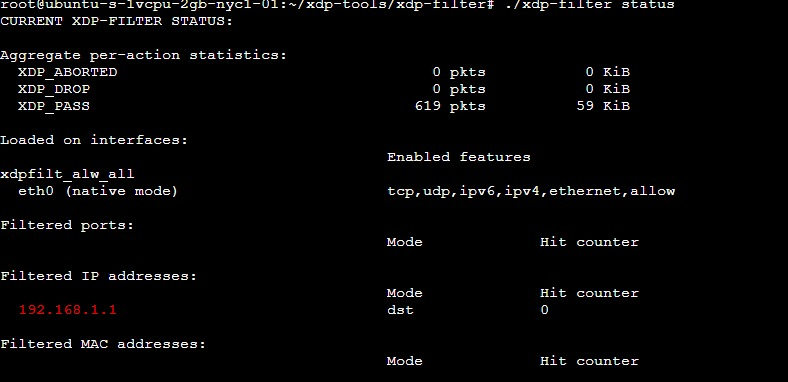
\includegraphics[width=0.8\textwidth]{../images/xdp-filter-ip.jpeg}
    \caption{Example output of xdp-filter filtering packets by IP address}
    \label{fig:xdp-filter-example}
\end{figure}

To load the xdp-filter program on a specific interface, use the following command:
\begin{verbatim}
    ./xdp-filter load eth0
\end{verbatim}
The figure \ref{fig:xdp-filter-load} shows the example output of xdp-filter loading the program on the eth0 interface.
\begin{figure}[H]
    \centering
    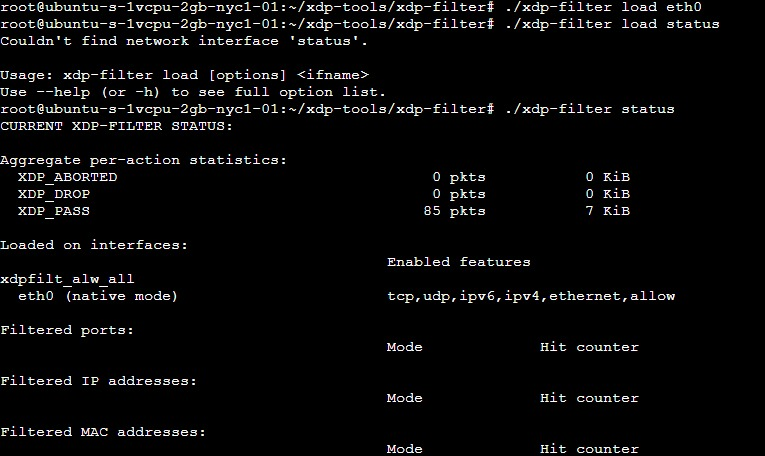
\includegraphics[width=0.8\textwidth]{../images/xdp-filter-load-eth0.jpeg}
    \caption{Example output of xdp-filter loading the program on the eth0 interface}
    \label{fig:xdp-filter-load}
\end{figure}

To poll for packets using xdp-filter, use the following command:
\begin{verbatim}
    ./xdp-filter poll
\end{verbatim}
The figure \ref{fig:xdp-filter-poll} shows the example output of xdp-filter polling for packets.
\begin{figure}[H]
    \centering
    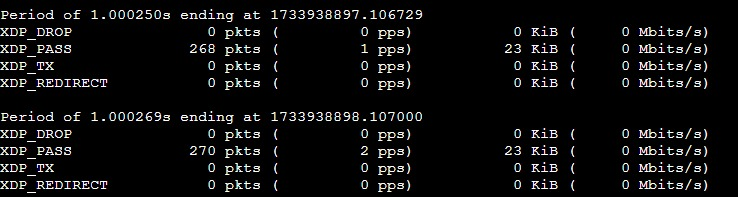
\includegraphics[width=0.8\textwidth]{../images/xdp-filter-poll.jpeg}
    \caption{Example output of xdp-filter polling for packets}
    \label{fig:xdp-filter-poll}
\end{figure}

To check all the available options for xdp-filter, use the following command:
\begin{verbatim}
    ./xdp-filter --help  or ./xdp-filter -h or ./xdp-filter
\end{verbatim}
The figure \ref{fig:xdp-filter-help} shows the available options for xdp-filter.
\begin{figure}[H]
    \centering
    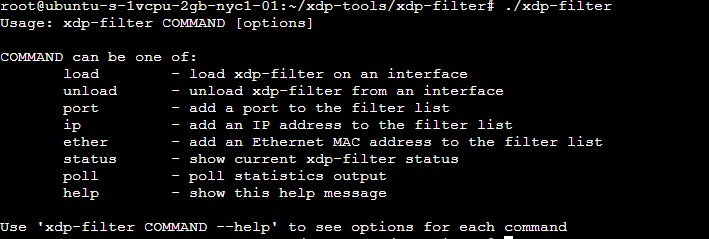
\includegraphics[width=0.8\textwidth]{../images/xdp-filter-help.jpeg}
    \caption{Available options for xdp-filter}
    \label{fig:xdp-filter-help}
\end{figure}

\subsection{xdp-dump}
The xdp-dump tool is used to dump packet data for analysis. Navigate to the xdp-dump directory:
\begin{verbatim}
cd xdp-tools/xdp-dump
\end{verbatim}

To dump packets for a specific interface, use the following command:
\begin{verbatim}
sudo ./xdp-dump -i eth0
\end{verbatim}
The figure \ref{fig:xdp-dump-example} shows the example output of xdp-dump showing dumped packet data over eth0 interface.
\begin{figure}[H]
    \centering
    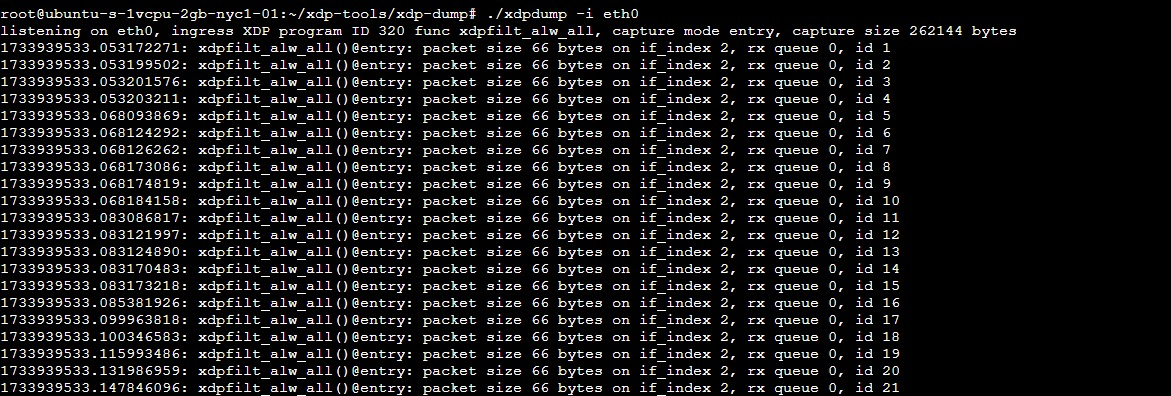
\includegraphics[width=0.8\textwidth]{../images/xdpdump-eth0.jpeg}
    \caption{Example output of xdp-dump showing dumped packet data over eth0 interface}
    \label{fig:xdp-dump-example}
\end{figure}

These tools provide powerful capabilities for filtering and analyzing network packets using XDP.

\section{Task 2: Real-time Cycle}
In this section, we describe the implementation of the real-time cycle for monitoring and analyzing network traffic. The backend logic is implemented using Django and the Django REST framework. The following functionalities are provided:

\subsection{Backend Implementation}
The backend logic is implemented in the \texttt{home/views.py} file. The main functionalities include capturing packets, predicting traffic, updating firewall status, and managing the monitoring process. Below is a brief overview of the key functions:

\begin{itemize}
    \item \textbf{home(request):} Renders the main index page with available network interfaces.
    \item \textbf{post\_flow(request):} Handles POST requests to receive flow data, make predictions, and update firewall status.
    \item \textbf{start\_interface(request):} Starts monitoring the specified network interface using cicflowmeter and updates configuration.
    \item \textbf{clear\_db(request):} Clears all entries in the FlowData database.
    \item \textbf{stop\_interface(request):} Stops the cicflowmeter process if it is running and updates configuration.
    \item \textbf{get\_data(request):} Retrieves flow data, blocked IPs, and monitoring settings, and returns them in the response.
\end{itemize}

\subsection{Real-time Monitoring and Analysis}
To achieve real-time monitoring and analysis, the following steps are performed:

\begin{itemize}
    \item Capture packets using cicflowmeter.
    \item Flowmeterize packets.
    \item Detect malicious packets with classifiers.
    \item Filter out malicious packets in real-time.
\end{itemize}

The backend logic ensures that the system can capture, analyze, and respond to network traffic in real-time, providing an effective solution for network monitoring and security.

\section{Task 3: Design front-end and interface}
For the front-end and interface design, we will use the following technologies:
\begin{itemize}
    \item \textbf{Django:} A high-level Python web framework that encourages rapid development and clean, pragmatic design.
    \item \textbf{HTML/CSS:} For designing the front-end interface.
    \item \textbf{JavaScript:} For adding interactivity to the front-end.
    \item \textbf{MySql:} For storing data and user information.
\end{itemize}

We designed a user-friendly interface that allows users to interact with the system, view real-time packet data, and manage the system's configuration.
Network flows list, live traffic, chart for normal and ddos packets, start/stop capturing, clean database, select interface, number of records, and Block/Unblock IP are the main features of the front-end interface.
The figure \ref{fig:front-end} shows the front-end interface of the system.
\begin{figure}[H]
    \centering
    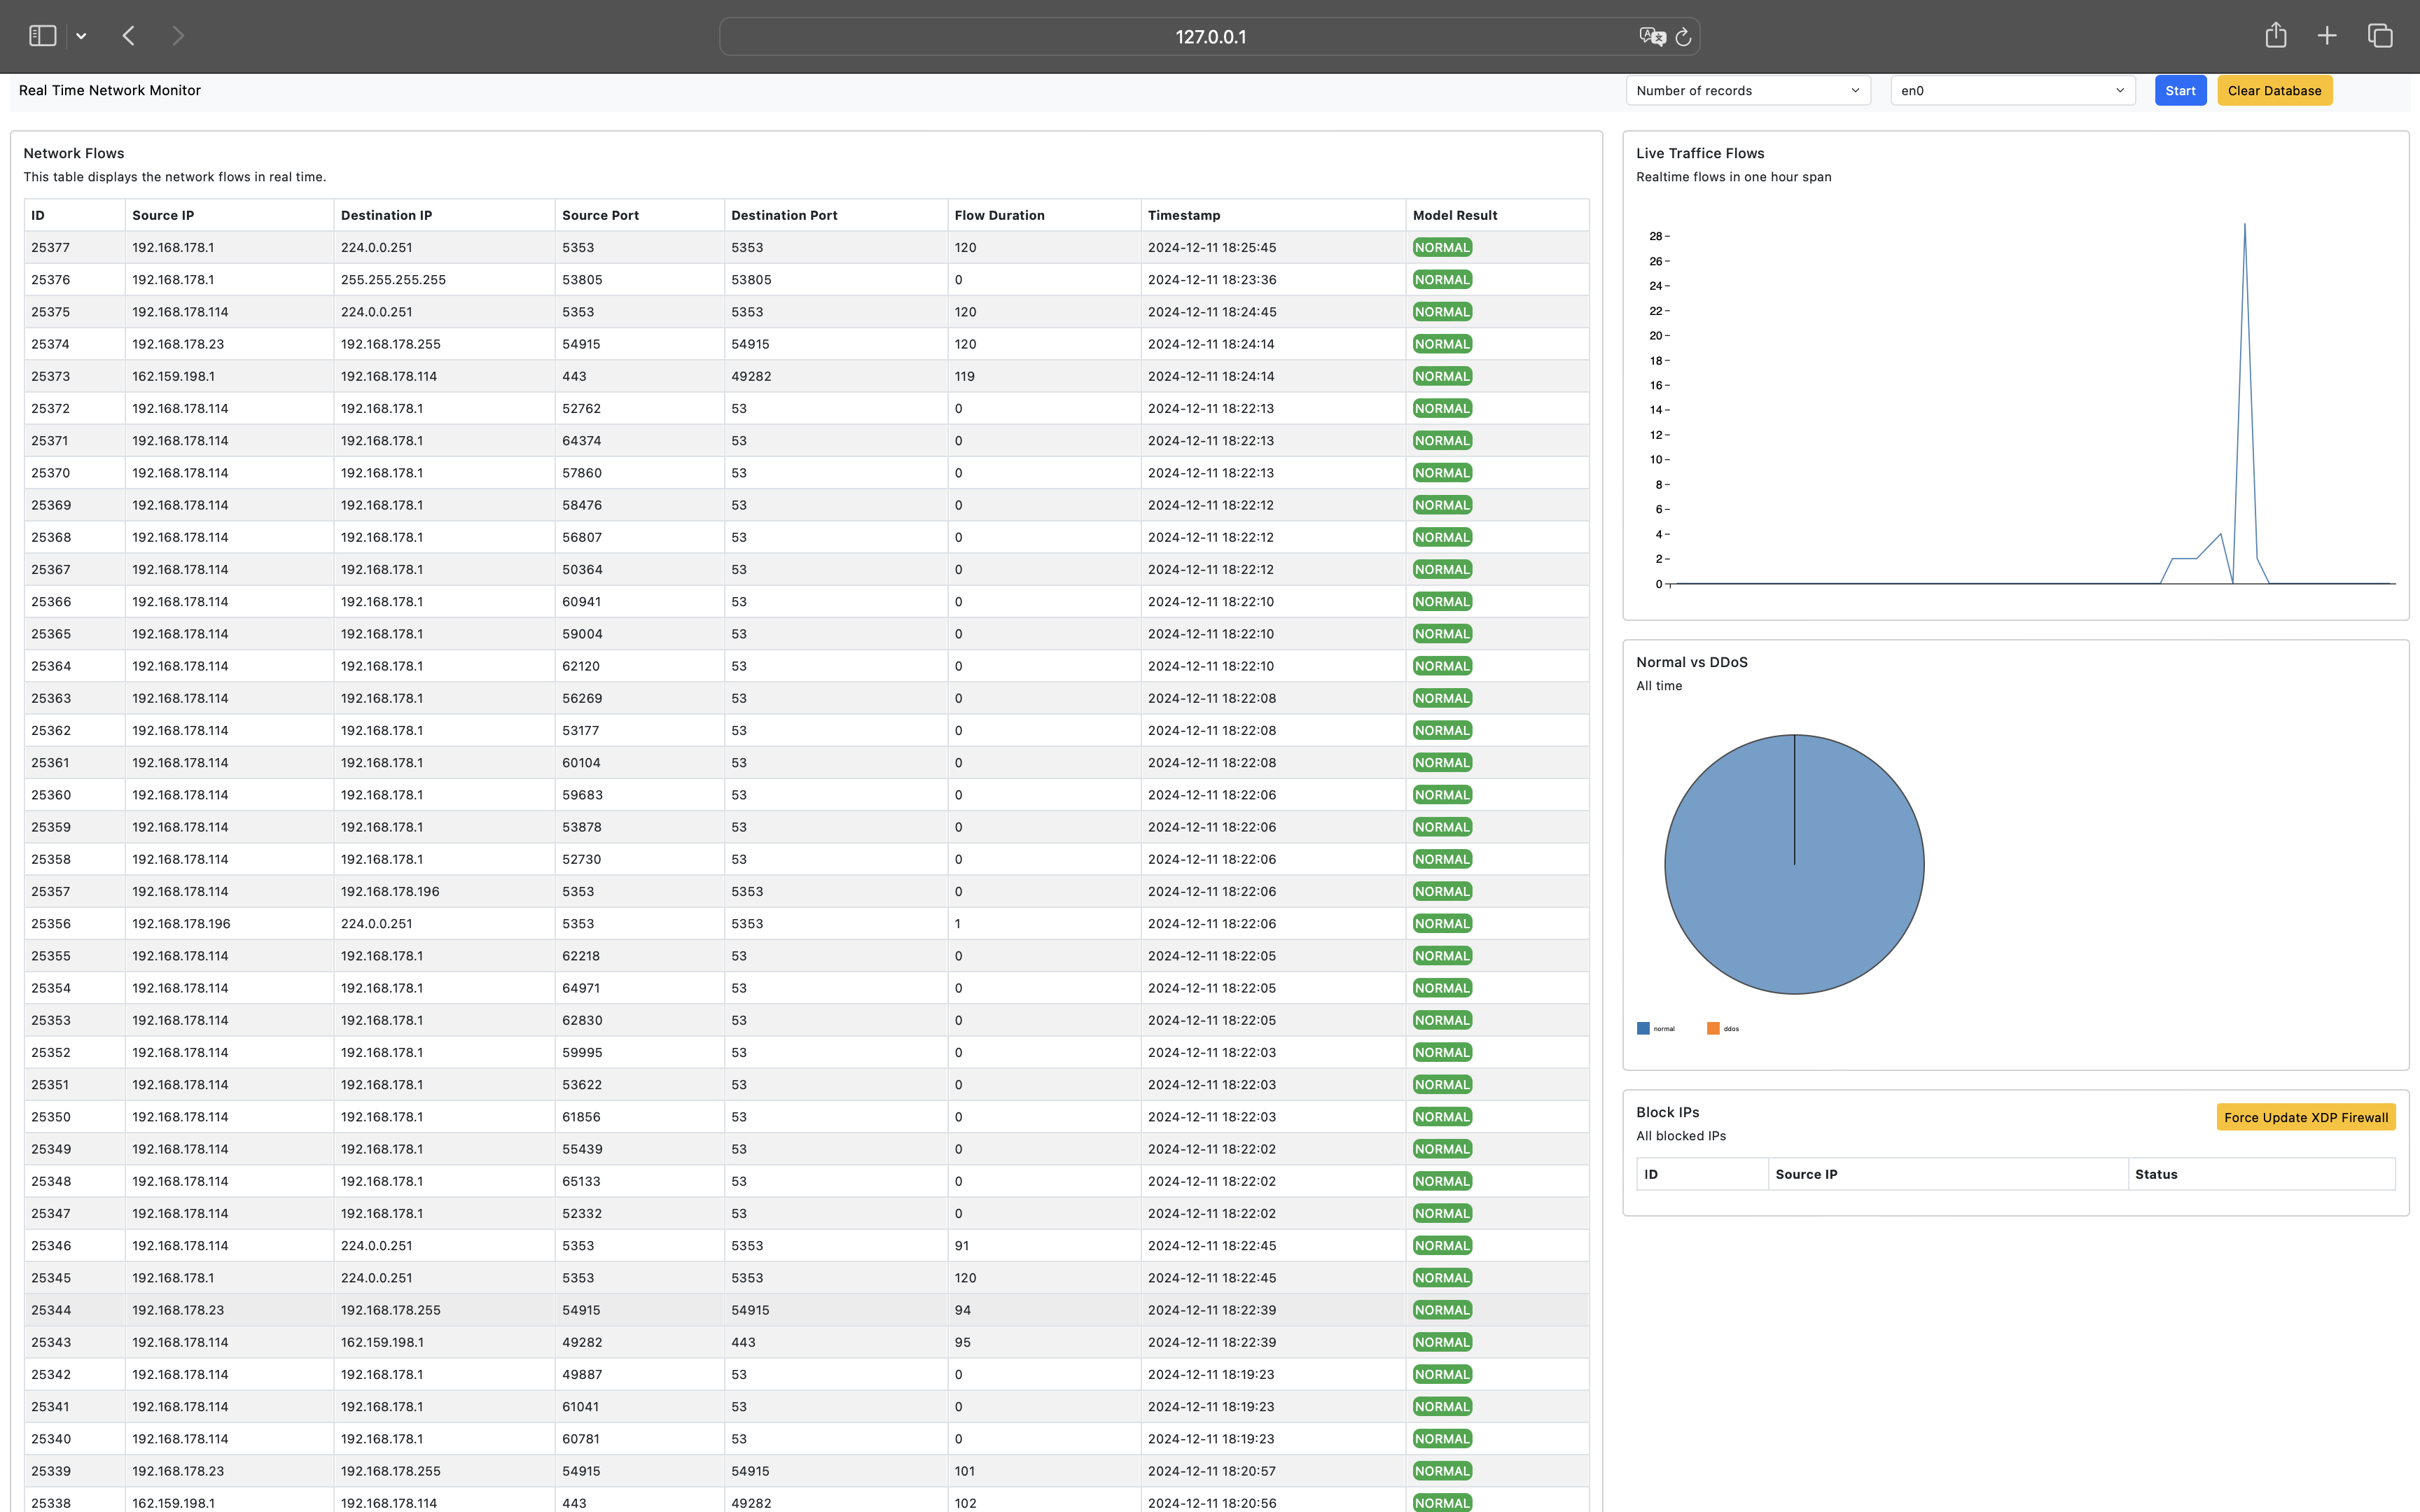
\includegraphics[width=0.8\textwidth]{../images/front-end.png}
    \caption{Front-end interface of the system}
    \label{fig:front-end}
\end{figure}
User by selecting an interface and clicking on the start button can start the packet capturing. 
The system will start capturing packets and show the live traffic in the live traffic section. 
The figure \ref{fig:live-traffic} shows the live traffic in the live traffic section.
\begin{figure}[H]
    \centering
    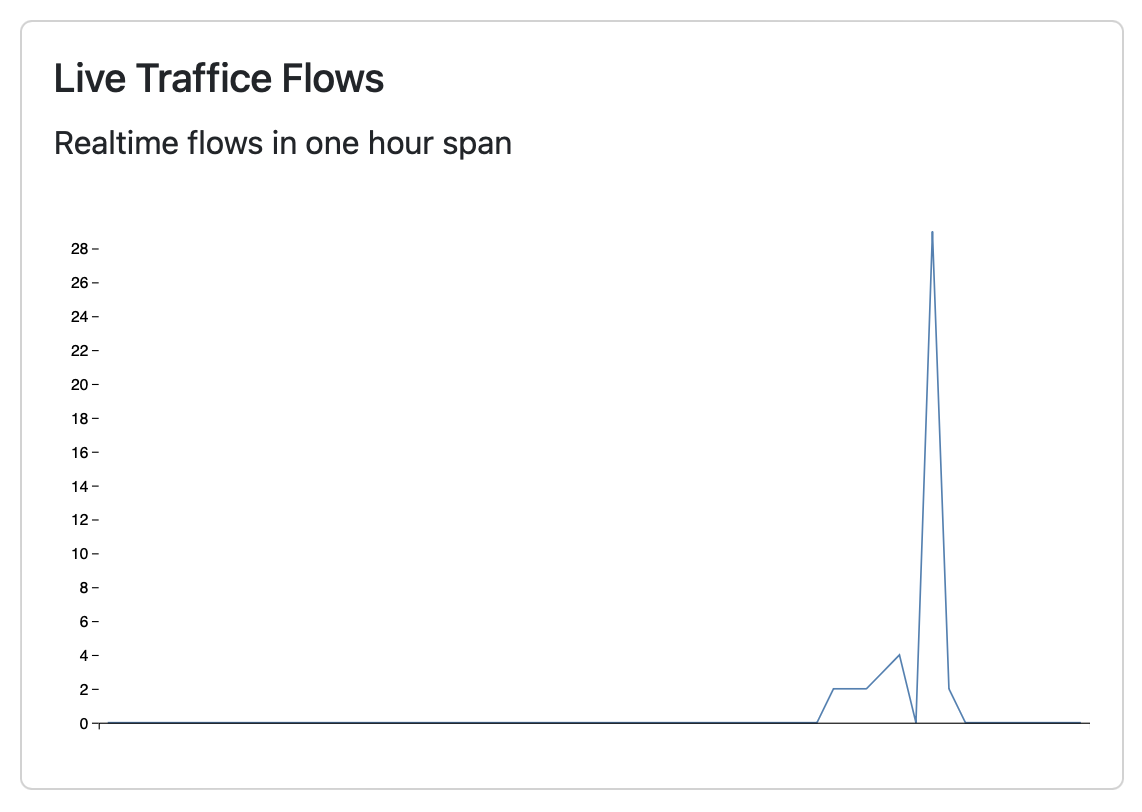
\includegraphics[width=0.8\textwidth]{../images/live-traffic.png}
    \caption{Live traffic in the live traffic section}
    \label{fig:live-traffic}
\end{figure}
The system will also show the network flows list with ID, Source IP, Destination IP, Source Port, Destination Port, Flow Duration, TimeStamp, Model Result. Figure \ref{fig:network-flows} shows the network flows list.
\begin{figure}[H]
    \centering
    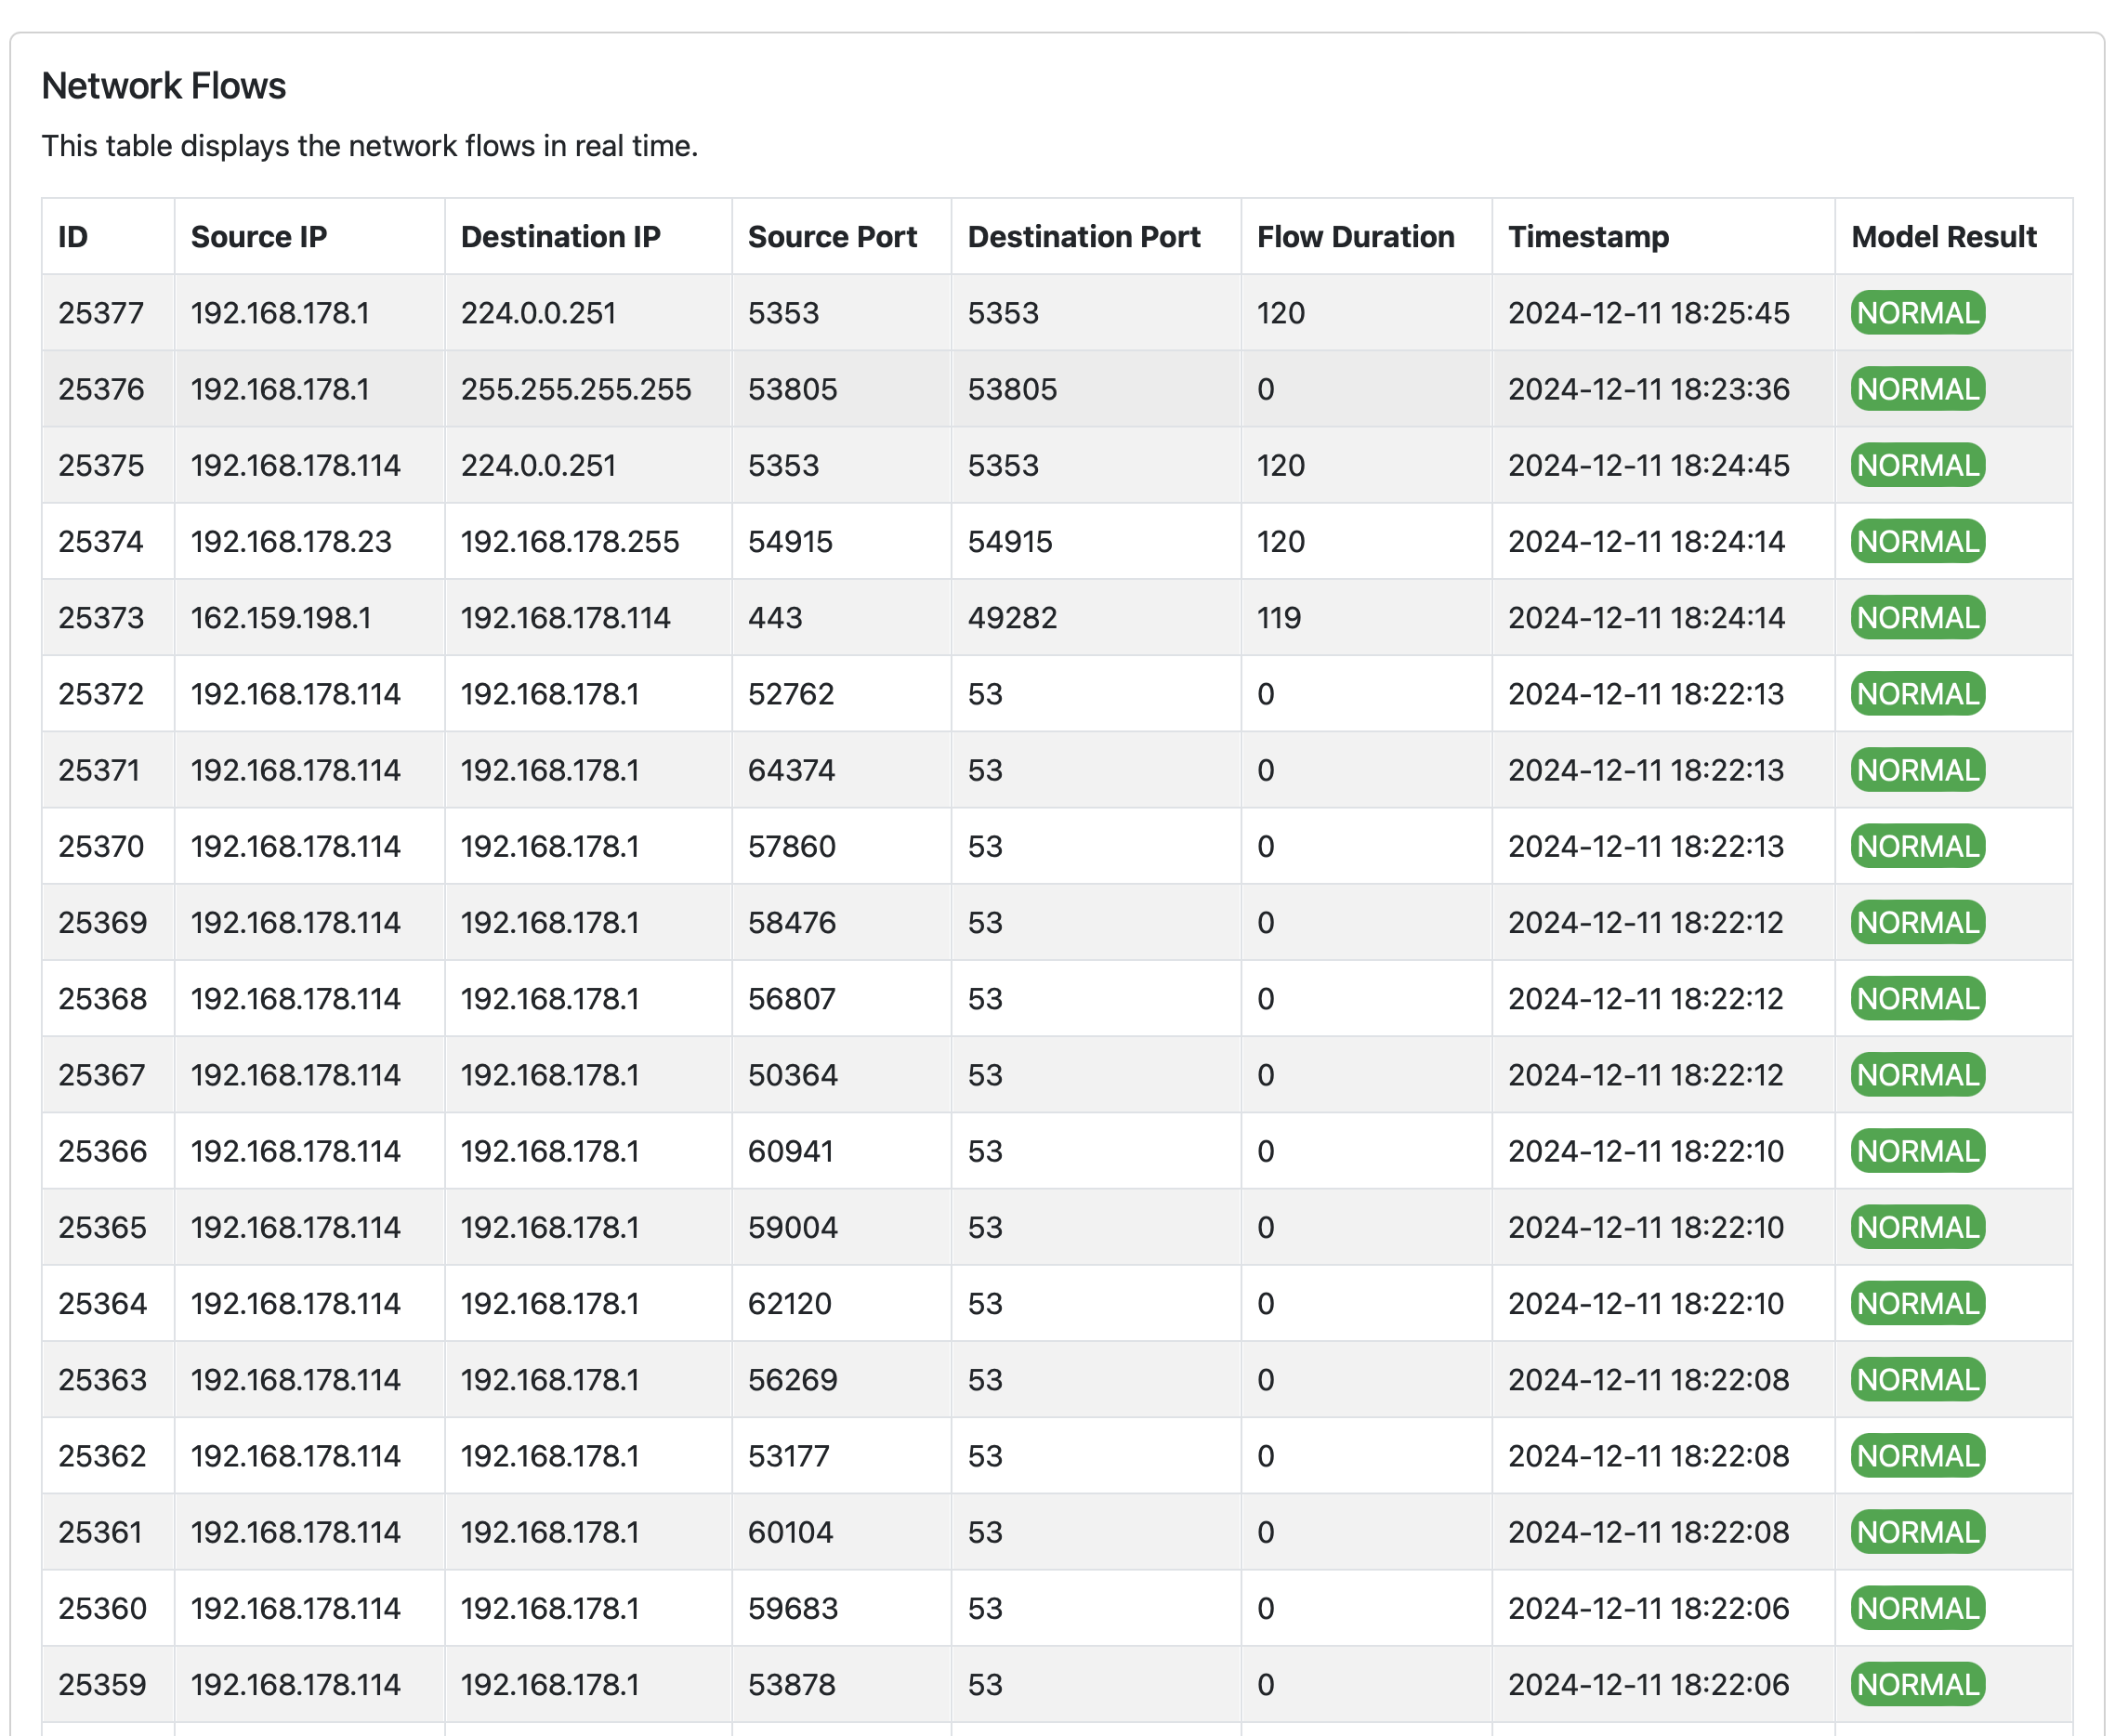
\includegraphics[width=0.8\textwidth]{../images/network-flows.png}
    \caption{Network flows list}
    \label{fig:network-flows}
\end{figure}
To have a comparison between normal and ddos packets, the system will show a pie chart for normal and ddos packets. The figure \ref{fig:normalDDOs} shows the chart for normal and ddos packets.
\begin{figure}[H]
    \centering
    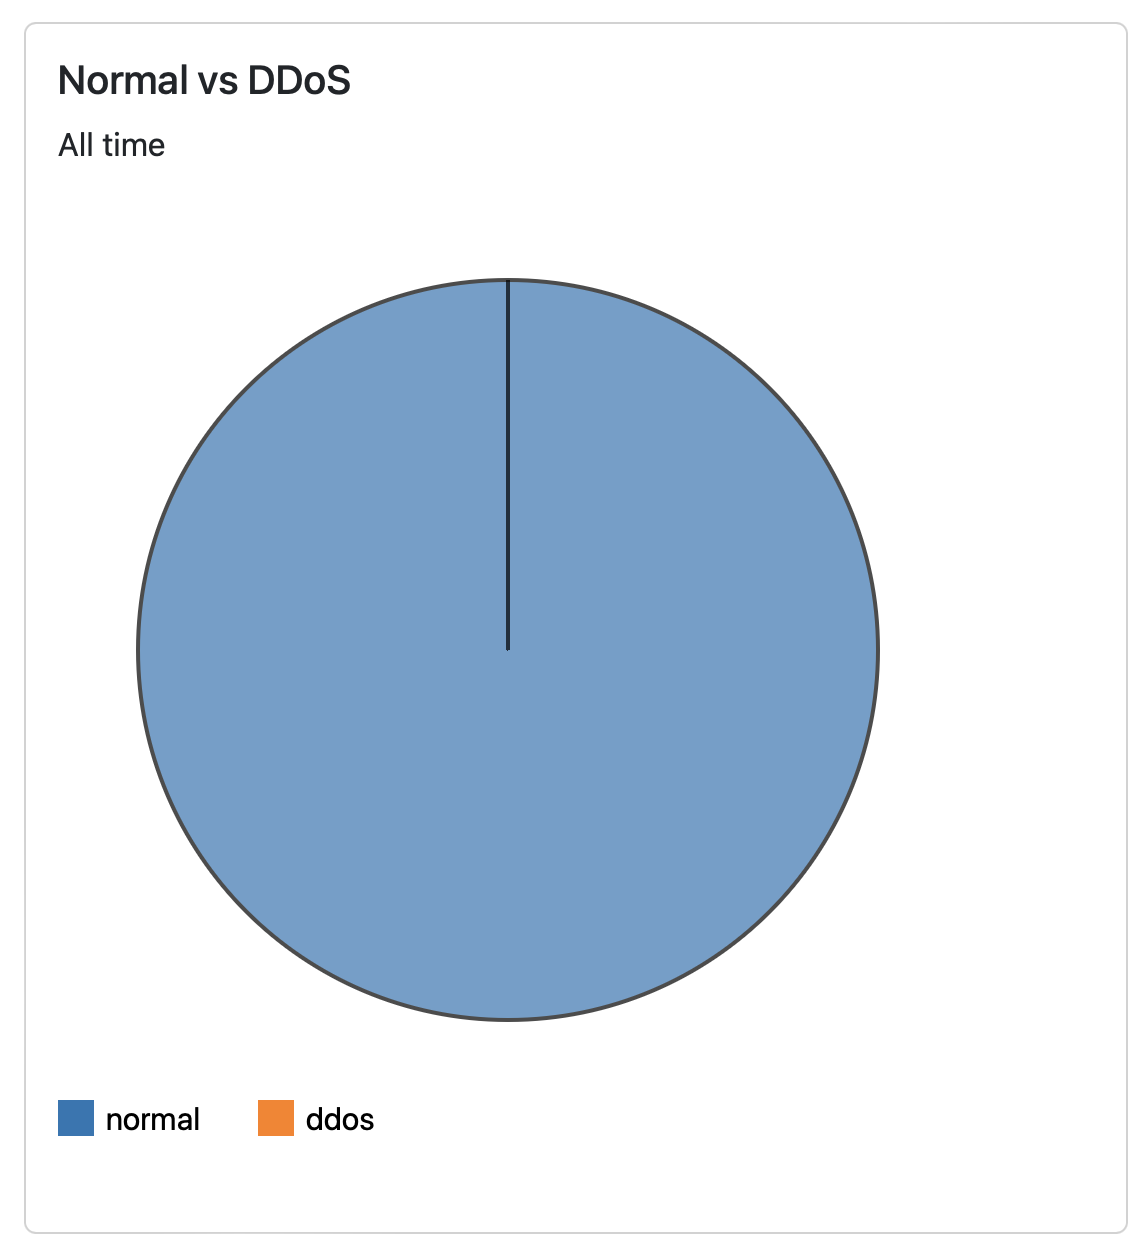
\includegraphics[width=0.8\textwidth]{../images/packatecomparison.png}
    \caption{Chart for normal and ddos packets}
    \label{fig:normalDDOs}
\end{figure}

The user can also block or unblock an IP address by clicking on the Block/Unblock IP button. This functionality has been achieved by using XDP library. The figure \ref{fig:block-unblock} shows the block/unblock IP functionality.
\begin{figure}[H]
    \centering
    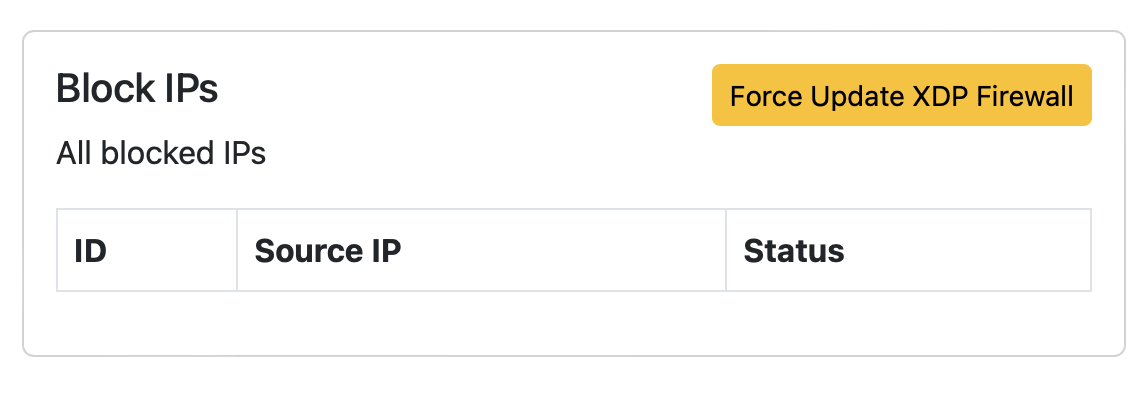
\includegraphics[width=0.8\textwidth]{../images/block-unblock.png}
    \caption{Block/Unblock IP functionality}
    \label{fig:block-unblock}
\end{figure}


\section{Task 4: Containerization \& Orchestration}

To run the system in a containerized environment, we will use Docker and Docker Compose.
\subsection{Containerization with Docker}
To containerize the system, follow these steps:

\begin{enumerate}
    \item \textbf{Install Docker:} First, install Docker on your system by following the instructions at \url{https://docs.docker.com/get-docker/}.
    \item \textbf{Build the Docker image:} Run the following command in the terminal to build the Docker image:
    \begin{verbatim}
    docker build -t {group2-rtnm} .
    \end{verbatim}
    \item \textbf{Run the Docker container:} Once the image is built, run the container using the following command:
    \begin{verbatim}
    docker run -p 8000:8000 group2-rtnm
    \end{verbatim}
\end{enumerate}

\subsection{Orchestration with Docker Compose}
To orchestrate the containers, follow these steps:

\begin{enumerate}
    \item \textbf{Install Docker Compose:} Ensure Docker Compose is installed on your system. If not, follow the instructions at \url{https://docs.docker.com/compose/install/}.
    \item \textbf{Start the services:} Run the following command to start the services defined in the \texttt{docker-compose.yml} file:
    \begin{verbatim}
        // For the first time
    docker-compose up --build
        // Other times
    docker-compose up
    \end{verbatim}
\end{enumerate}

The system will now be running in a containerized environment, allowing for easy deployment and management.
To access the system, open a web browser and navigate to \url{http://localhost:8000/}.
% \chapter{Results}\label{chap:results}

% \chapter{Discussion}\label{chap:discussion}


% -- Appendix (optional)
% \begin{appendices}
%     % !TeX spellcheck = en_US
% !TeX encoding = UTF-8
\chapter{Code}

\chapter{Math}

\chapter{Dataset}
% \end{appendices}
% \newpage


%%%%%%%%%%%%%%%%%%%%%%%%%%%%%%%%%%%%%%%%%%%%%%%%%%%%%%%%%%%%%%%%%%%%%%%%%%%%%%%%%%%%%%%%%
\backmatter

% -- Bibliography
\printbibliography

% -- Eidesstattliche Erklärung (= Affadavit)
% % !TeX spellcheck = de_DE
% !TeX encoding = UTF-8
\begin{german}
\chapter{Eidesstattliche Erklärung}

	Hiermit versichere ich, dass ich diese \thesisType{} selbstständig und ohne Benutzung anderer als der angegebenen Quellen und Hilfsmittel angefertigt habe und alle Ausführungen, die wörtlich oder sinngemäß übernommen wurden, als solche gekennzeichnet sind, sowie, dass ich die \thesisType in gleicher oder ähnlicher Form noch keiner anderen Prüfungsbehörde vorgelegt habe.

	\vspace{3cm}

	Passau, \thedate

	\vspace{2cm}

	\parbox{8cm}{
		\hrule \strut \theauthor
	}
\end{german}



\end{document}